% !TeX spellcheck = fr_FR
\chapter{Chapitre 1 : Phénomène physique}

%TODO explain light in general ?

\section{La lumière Cherenkov}

L'effet Cherenkov a lieu lorsqu'une particule chargée électriquement traverse un milieu diélectrique transparent
en excédant la vitesse maximale de la lumière dans ce même milieu. 
Lors de son passage, cette particule va exciter les autres particules du milieu et produire une réaction en chaîne.
Cette dernière va donc créer un cône de particules tel que des électrons, positrons ou photons et même des particules élémentaires nommées hadrons.
Cet effet est similaire au bang supersonique lorsque des objets dépassent le mur du son mais dans le spectre électromagnétique.
Le cas le plus connu de cet effet est celui qui peut être observé autour des réacteurs nucléaires, dû à la lumière bleue qu'il engendre.

\begin{figure}[tbph!]
	\centering
	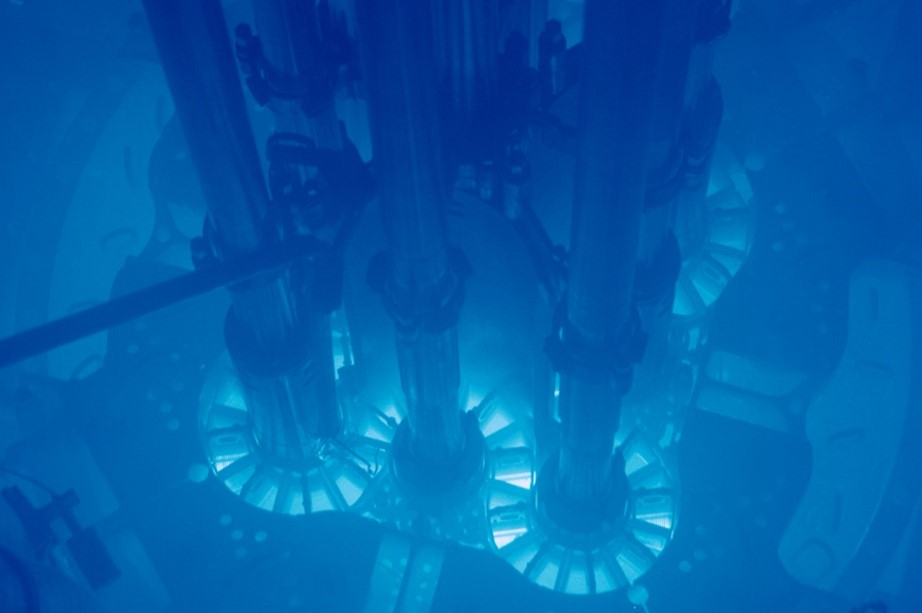
\includegraphics[width=0.6\linewidth]{cherenkov_radiation}
	\caption[Advanced Test Reactor core, Idaho National Laboratory]{Advanced Test Reactor core, Idaho National Laboratory. Source : \cite{CherenkovRadiation}}
\end{figure}

%TODO better redaction ?
L'intensité de la lumière est communément quantifiée en électron-volt ou eV.
Cette unité représente l'énergie cinétique gagnée lorsqu'un électron voit son énergie potentielle augmentée d'un Volt dans le vide.
%END TODO

La lumière Cherenkov atmosphérique peut produire deux types de pluies différentes : les pluies purement \gls{em}
composées uniquement d'électrons, positrons et photons ainsi que les pluies hadroniques qui elles sont composées de hadrons chargés électriquement, comme des protons.
\newpage
\begin{figure}[tbph!]
	\centering
	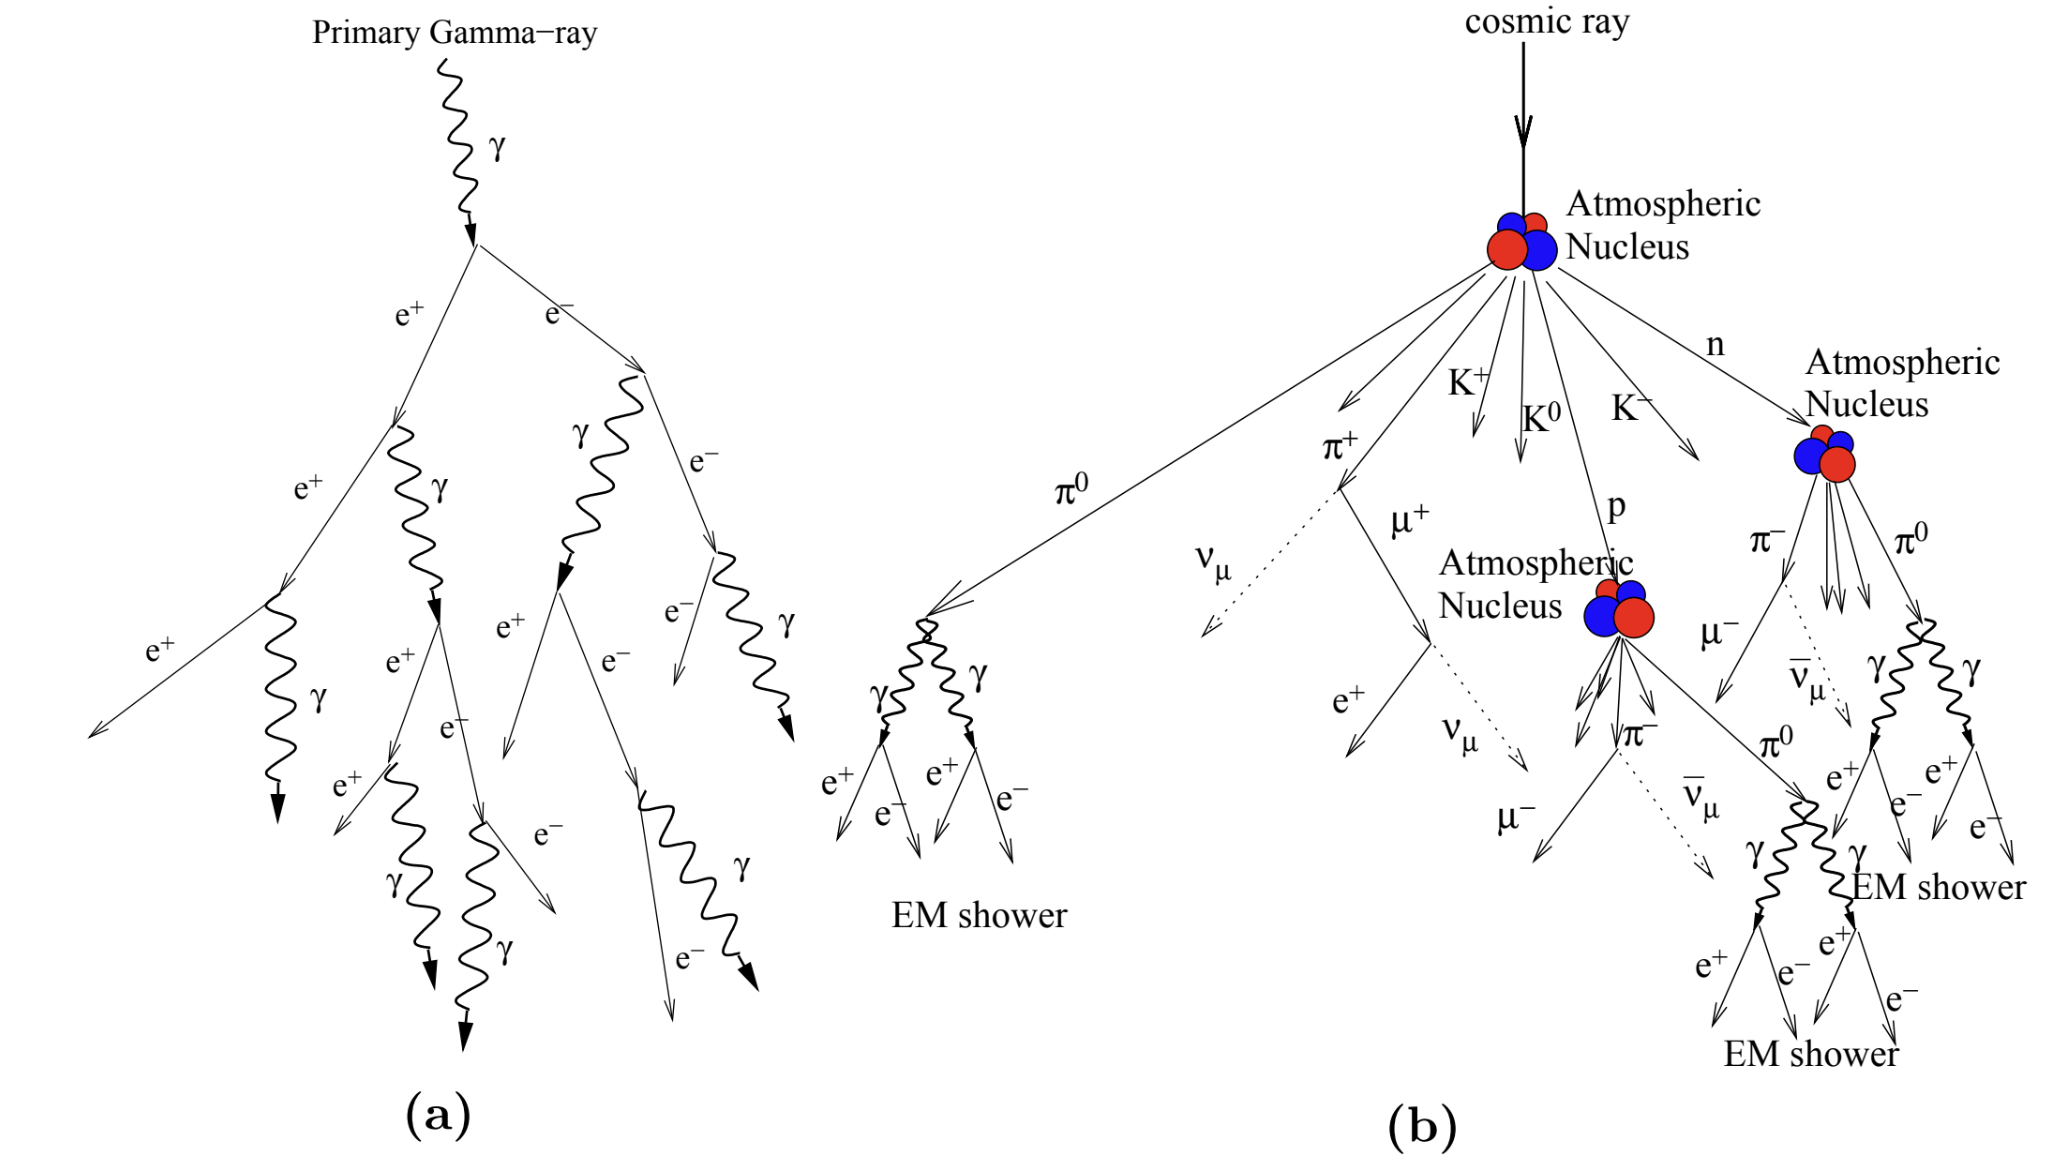
\includegraphics[width=\textwidth]{cherenkov_showers.png}
	\caption[Diagramme de pluies EM et hadroniques]{Diagramme de pluies électromagnétiques pures (a) et pluies hadroniques (b). Source : I. Oya Vallejo. “Observation of active galactic nuclei with the Magic telescope”. UCM. PhD thesis. 2010.}
\end{figure}

Les pluies hadroniques sont généralement plus puissantes que des pluies \gls{em} et ont voit aussi qu'elles se décomposent au fur et à mesure en pluies \gls{em}.
Pour les pluies \gls{em}, la production d'électrons et de positrons se fait via deux principes physiques : la production de paires et par rayonnement continu de freinage.
La production de paires se produit lorsqu'une particule chargée à haute énergie interagit aux abords du noyau d'une autre particule.
Suite à cette interaction un électron et un positron sont produits. Ces deux particules vont ensuite créer à leur tour des photons 
lorsqu'elles ralentissent autour d'autres noyaux. Ce ralentissement a comme conséquence de produire un photon.
\newpage
\begin{figure}[!tbp]
	\centering
	\begin{minipage}[b]{0.4\textwidth}
	  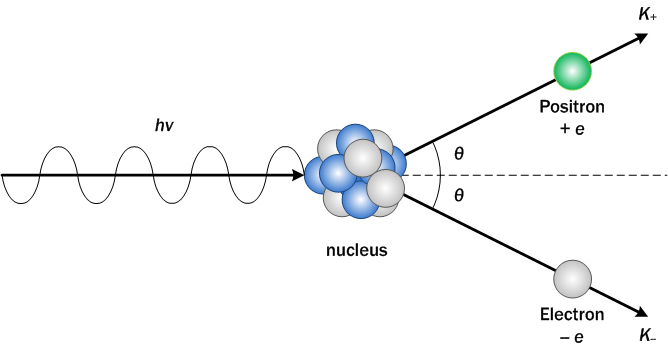
\includegraphics[width=\textwidth]{PairProduction.jpg}
	  \caption[Création de paires]{Diagramme de création de paires. Source : \cite{PairProduction}}
	\end{minipage}
	\hfill
	\begin{minipage}[b]{0.4\textwidth}
	  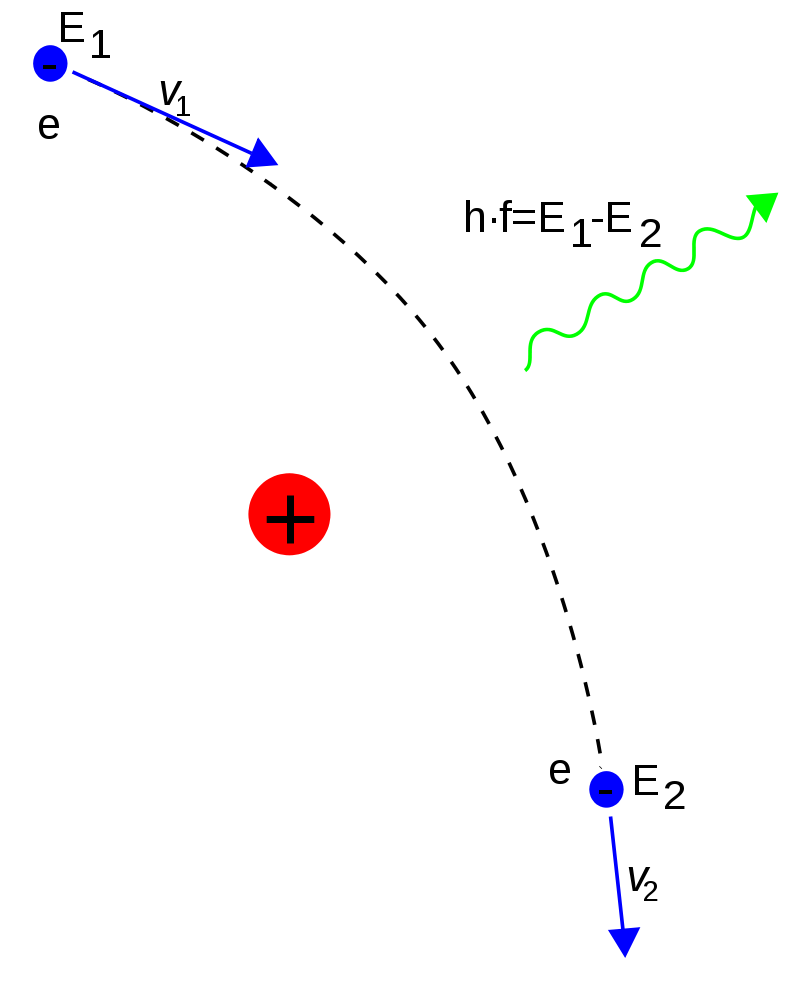
\includegraphics[width=\textwidth]{RayonnementContinuDeFreinage.png}
	  \caption[Rayonnement continu de freinage]{Diagramme de rayonnement continu de freinage. Source : \cite{Bremsstrahlung}}
	\end{minipage}
\end{figure}

L'intérêt scientifique se porte cependant plus sur les pluies \gls{em} pures à cause des rayons gamma qui débutent la réaction en chaîne.
Comparés aux particules chargées comme des protons, les rayons gamma eux ne sont pas déviés par les champs électriques ou magnétiques 
pendant leur trajet à travers les astres. En détectant ces pluies purement \gls{em}, on peut en déduire leur provenance beaucoup plus simplement 
que pour des pluies hadroniques où il faut prendre en compte les différentes interactions astronomiques et atmosphériques.

% TODO energy levels for gamma / hadronic split

\section{Méthodes de détection}
Les rayons gamma varient grandement en intensité de quelques MeV jusqu'à des dizaines de PeV et plus encore jusqu'au maximum ~100 EeV. \cite{TjarkPHD}
En fonction de l'énergie d'un rayon gamma, certaines techniques sont plus optimisées que d'autres, ici on retrouve les différentes techniques utilisées aujourd'hui :

% TODO Better explanation of physics for actual detection
% Chaque tube photomultiplicateur est capable de quantifier l'énergie reçue par des photons en entrée du capteur et il "stocke" cette valeur en tant que charge électrique. 
% En échantillonnant cette charge électrique a intervalle réguliers on retrouve une forme d'onde de l'amplitude détectée sur le temps.
%END TODO
\begin{table}[tbph!]
	\centering{
		\begin{tabular}{ |c|c|c|c| }
			\hline
			\textbf{Notation} & \textbf{Gamme d'énergie} & \textbf{Technique de détection} & \textbf{Emplacement} \\
			\hline
			LE & < 30 MeV & Photoélectrique, Compton & Espace \\
			\hline
			HE & 30 MeV à 100 TeV & Création de paires & Espace \\
			\hline
			VHE & 100 GeV à 30 TeV & Cherenkov (atmosphérique) & Terrestre \\
			\hline 
			UHE & 30 TeV à 30 PeV & Cherenkov (eau) & Terrestre \\
			\hline 
			EHE & > 30 PeV & Fluorescence, Hybride & Terrestre \\
			\hline 
		\end{tabular}
		\caption[Techniques de détection en fonction de la classification énergétique des rayons gamma]{Techniques de détection en fonction de la classification énergétique des rayons gamma. Source : \cite{TjarkPHD} p. 17}
	}
\end{table}

\section{Astronomie gamma existante}
\subsection{INTEGRAL}
En l'an 2002, l'agence spatiale européene a lancé le satellite INTEGRAL qui est le premier à avoir observé les spectres \gls{em} visible, x-ray et gamma en simultané.
Concernant les rayons gamma, ce satellite est équipé de deux capteurs englobant la plage de rayons gamma \gls{le} de ~15keV à ~10MeV \cite{IntegralSpecs} 

\begin{figure}[tbph!]
	\centering
	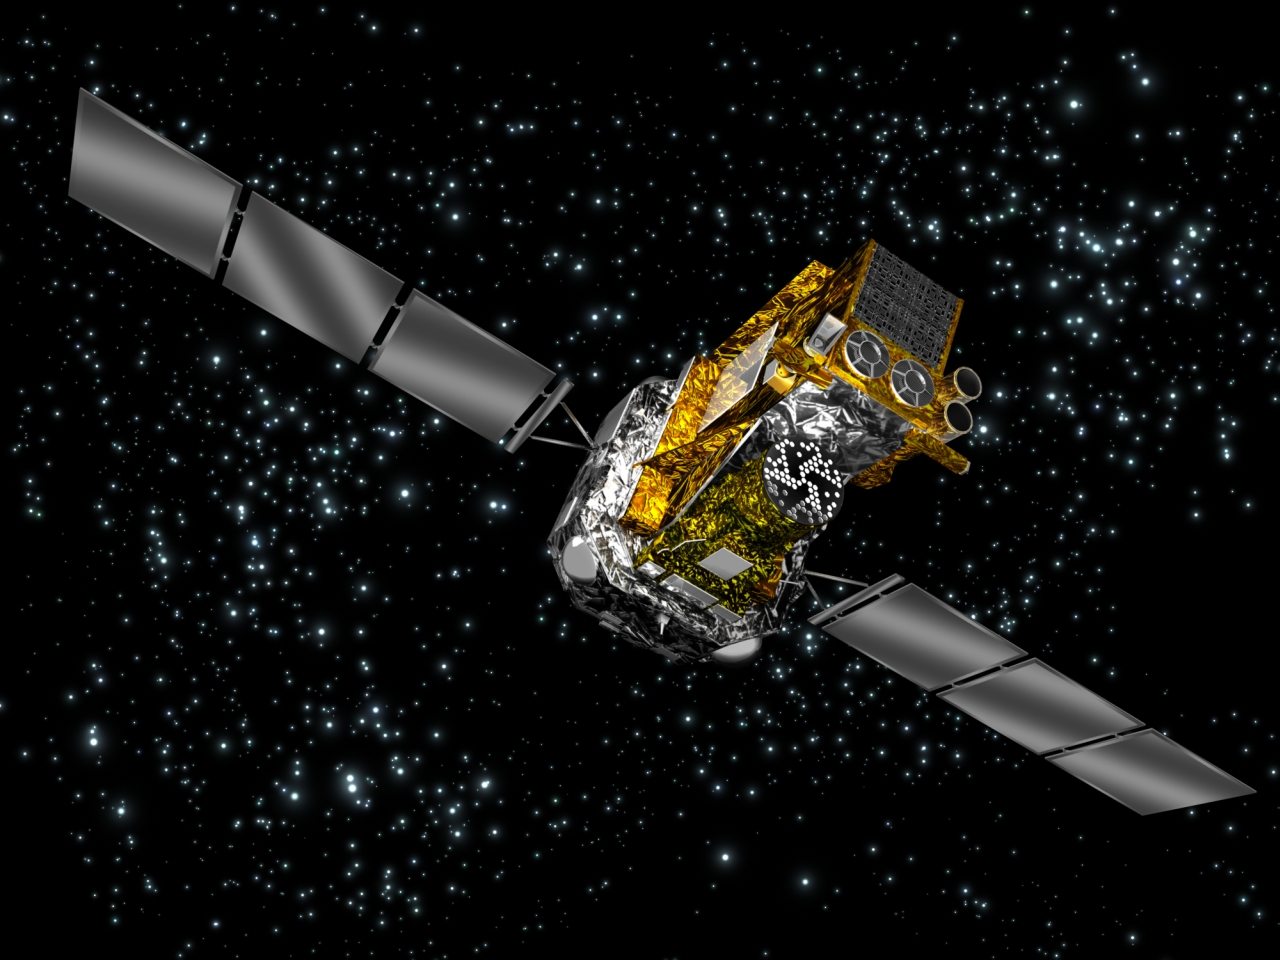
\includegraphics[width=0.4\linewidth]{Integral}
	\caption[Illustration du satellite INTEGRAL]{Illustration du satellite INTEGRAL. Source : \cite{IntegralImage}}
\end{figure}

\subsection{Fermi-LAT}
Le satellite Fermi a été développé par la \gls{nasa} en collaboration avec des institutions
françaises, allemandes, japonaises, italiennes et suédoises. Il a été envoyé en orbite en 2008 et il est en opération depuis lors. \cite{Fermi}
Il transporte deux instruments de mesures : le Large Area Telescope (20 MeV à > 300 GeV) et le Gamma-ray Burst Monitor (8 keV à 40 MeV).

Le détecteur fonctionne via la détection de production par paires à l'intérieur du détecteur après une collision d'un photon.
Les trajectoires et l'énergie dégagée par cet impact ressemble aux expériences des accélérateurs de particules.

L'observatoire fonctionne normalement en un mode de découverte qui scanne tout le spectre gamma du ciel.
Il est capable de scanner l'entièreté du ciel en seulement deux orbites.
Il a par exemple découvert les bulles de Fermi qui sont d'immenses sources de rayons gamma dans notre Voie lactée. 
Celles-ci proviendraient de grandes décharges d'énergie émises par le trou noir central de la galaxie il y a de cela plusieurs millions d'années.

\begin{figure}[tbph!]
	\centering
	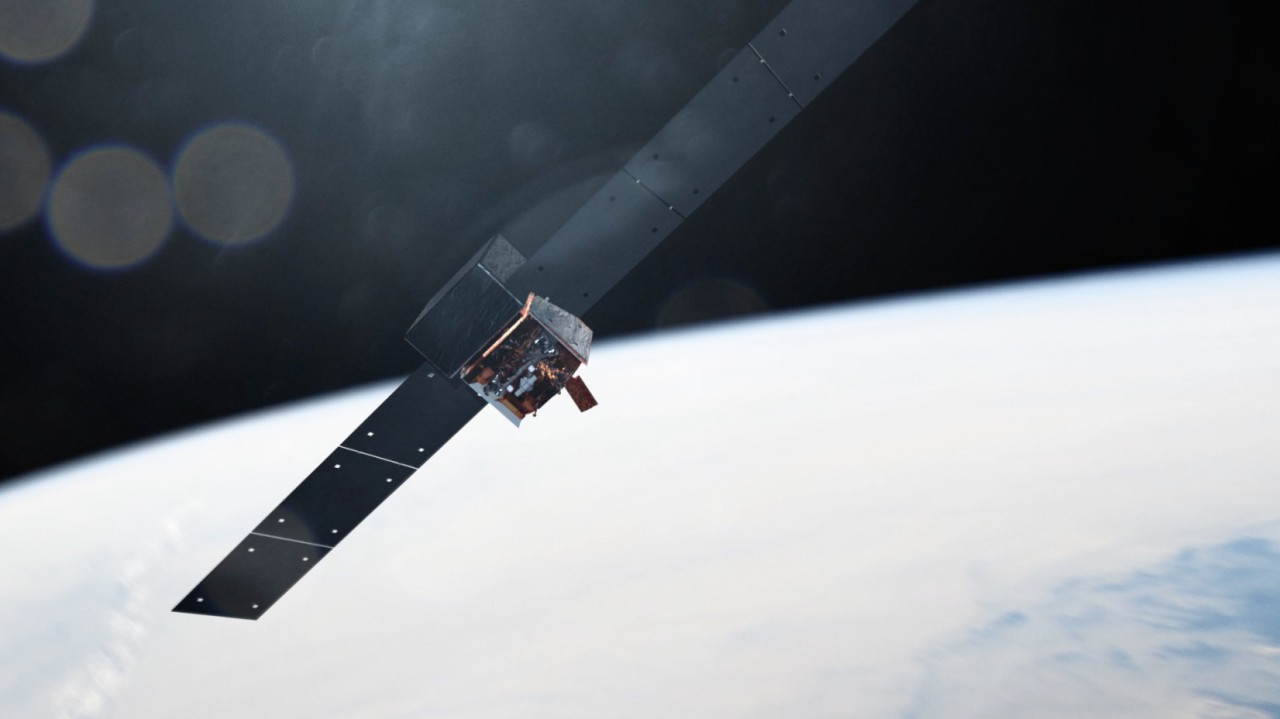
\includegraphics[width=0.5\linewidth]{fermi.jpg}
	\caption[Illustration du Fermi Gamma-ray Space Telescope en orbite]{Illustration du Fermi Gamma-ray Space Telescope en orbite. Source : \cite{FermiImage}}
\end{figure}

\subsection{MAGIC}
\textbf{MAGIC} est une installation de deux télescopes \gls{iact} complétée en 2009 à l'observatoire "Observatorio del Roque de los Muchachos" situé à La Palma aux îles
Canaries a une altitude d'environ 2200m. \cite{Magic}

Les télescopes ont été conçus pour étudier les rayons gamma \gls{vhe} de 30GeV à 100 TeV grace à leurs miroirs de 17m de diamètre qui réfléchissent la lumière dans
une grille hexagonale de 1039 tubes photomultiplicateurs, ce qui leur permet de visualiser le ciel avec un champ de vision du ciel de 3,5°.

\begin{figure}[tbph!]
	\centering
	\includegraphics[width=0.6\linewidth]{MAGIC.jpg}
	\caption[Photo des deux télescopes MAGIC]{Photo des deux télescopes MAGIC. Source : \cite{MagicImage}}
\end{figure}

\subsection{H.E.S.S.}
Le \textbf{High Energy Stereoscopic System} était initialement une installation de 4 télescopes de 12m formant un carré de 120m de côté rendu opérationnel en 2004 dans la région de Khomas en Namibie.
En 2012, un 5ème télescope de 28m et 580 tonnes a été ajouté au centre de ce carré, augmentant la sensibilité en la résolution angulaire du système. \cite{Hess}

Les quatre télescopes aux extrémités ont un champ de vision de 5° et sont équipés de caméras composées de 960 tubes photomultiplicateurs.
Le télescope central possède aussi une caméra composée de 2048 photomultiplicateurs avec un champ de vision de 3,2°.

\begin{figure}[tbph!]
	\centering
	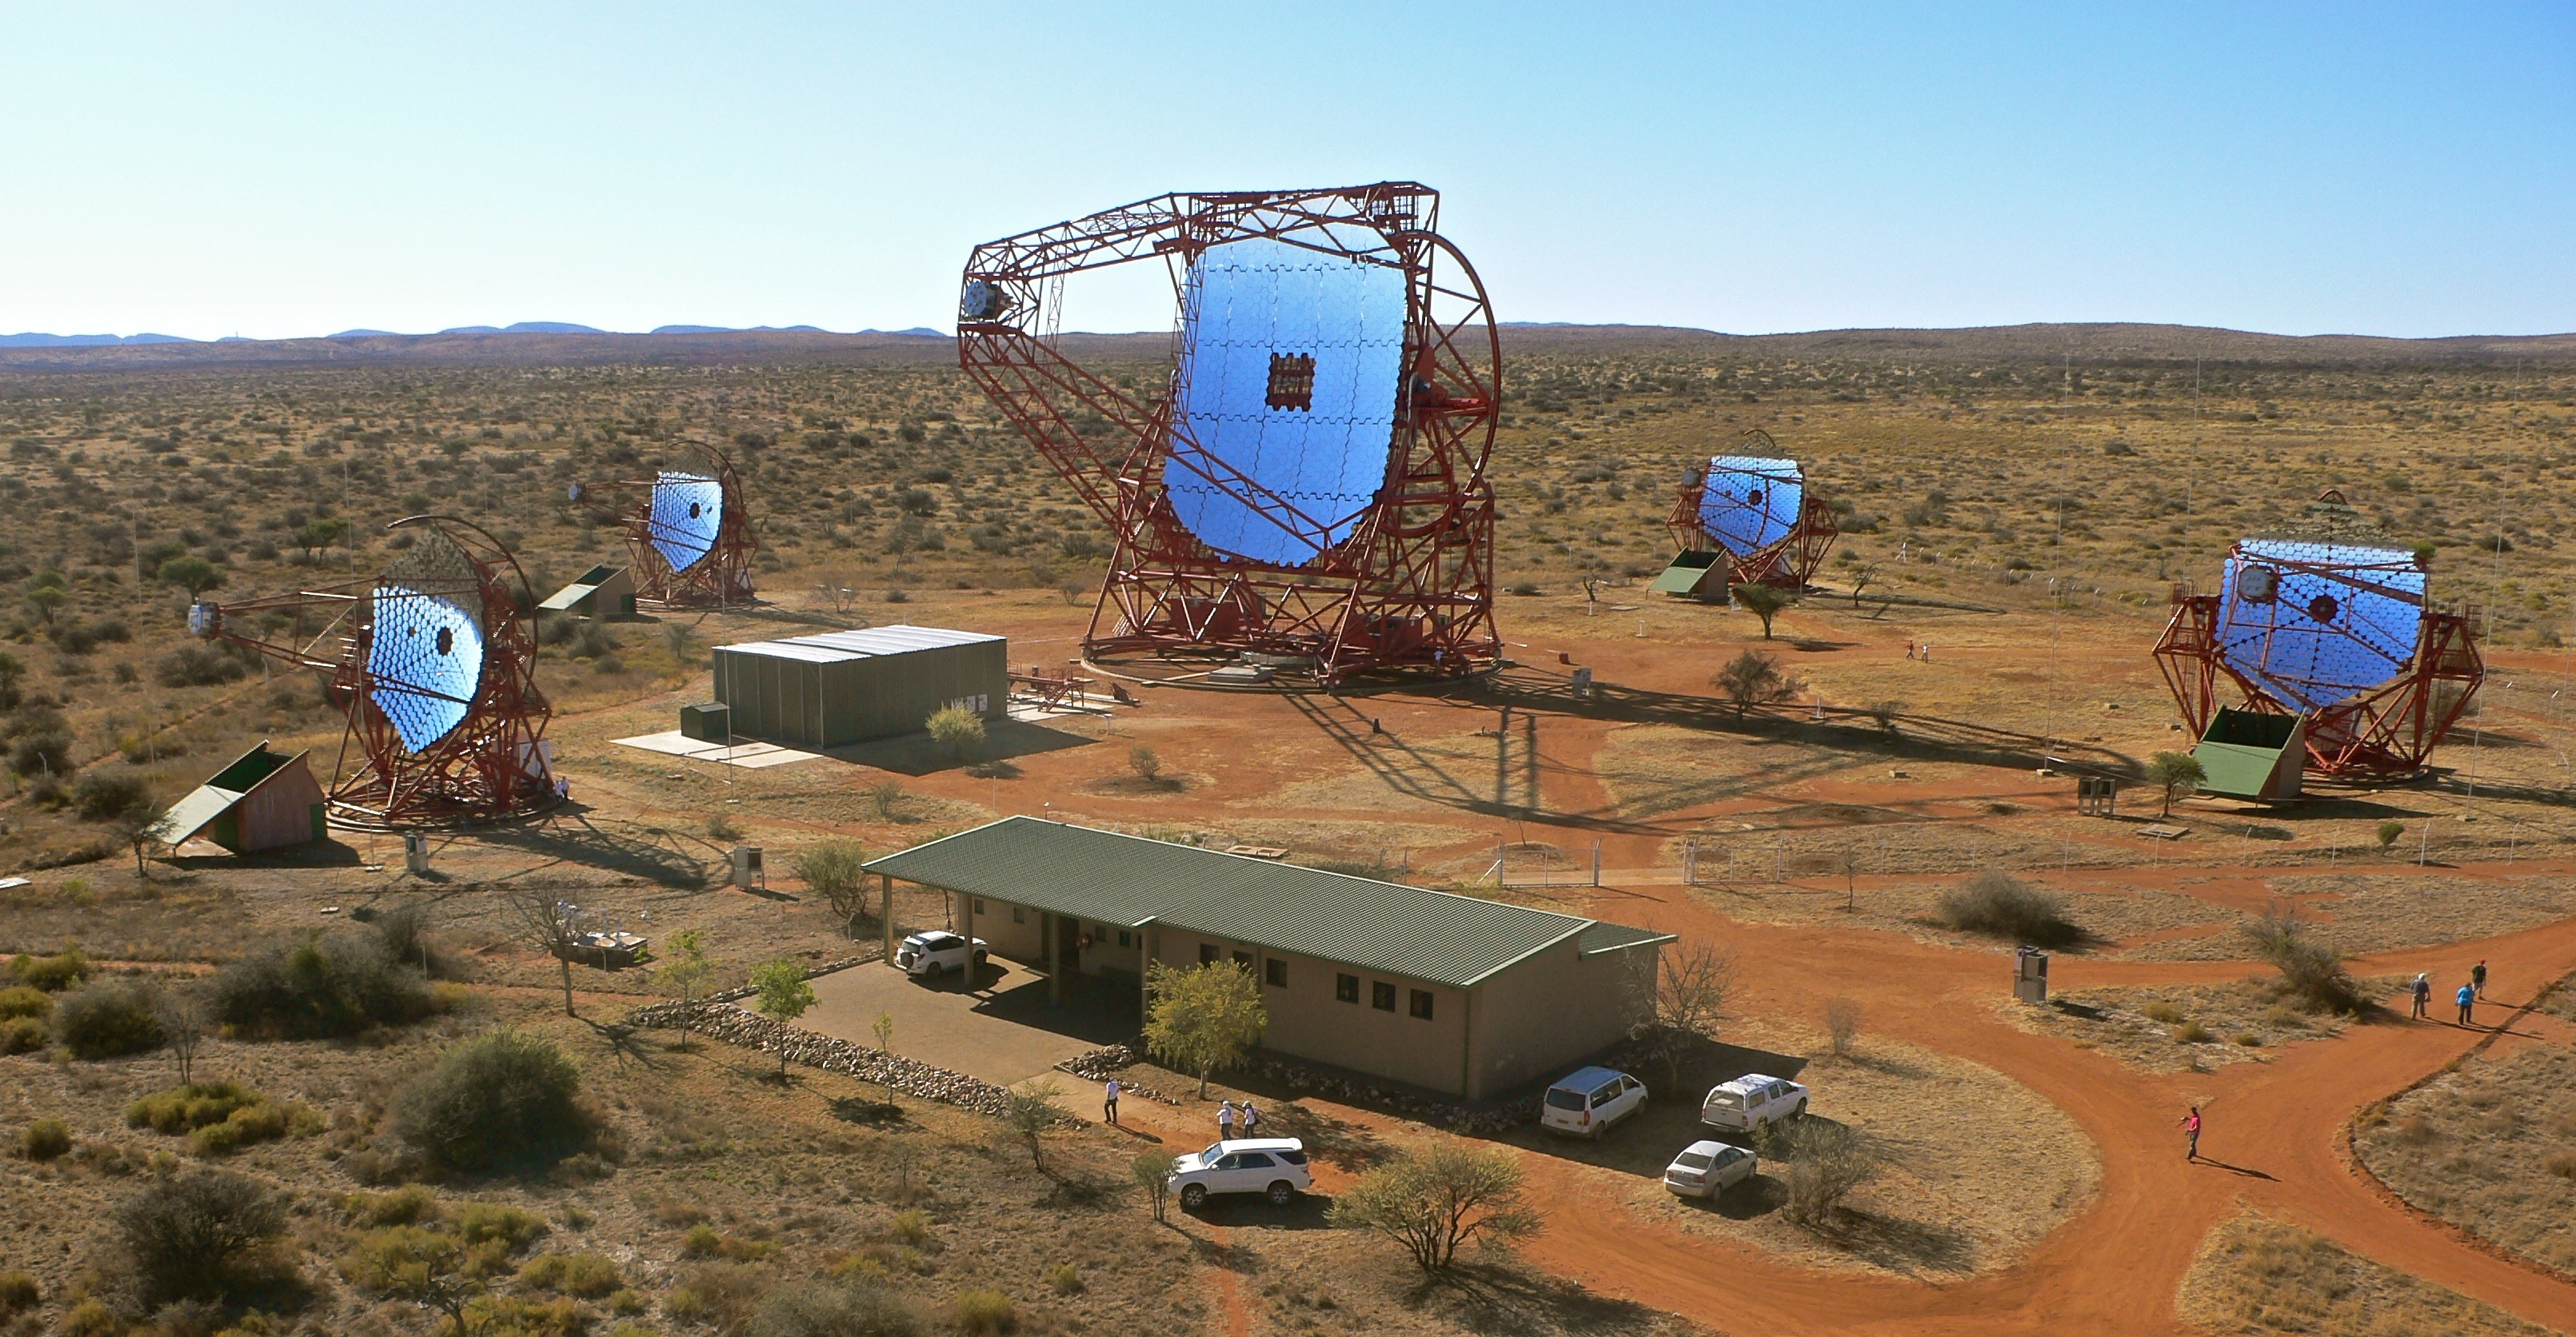
\includegraphics[width=0.6\linewidth]{hess.jpg}
	\caption[Photo de l'installation H.E.S.S]{Photo de l'installation H.E.S.S. Source : \cite{HessImage}}
\end{figure}

\subsection{VERITAS}
Le \textbf{Very Energetic Radiation Imaging Telescope Array System} est un projet financé par les USA, le Canada et l'Allemagne installé au Fred Lawrence Whipple Observatory dans l'Arizona.
Il est composé de quatre télescopes de 12m d'ouverture avec des caméras chacune composées de 499 tubes photomultiplicateurs. \cite{Veritas} 
L'installation a pour but d'étudier les rayons gamma \gls{vhe} entre 50GeV et 50TeV et a notamment été utilisée pour complémenter la mission Fermi de la \gls{nasa}.

\begin{figure}[tbph!]
	\centering
	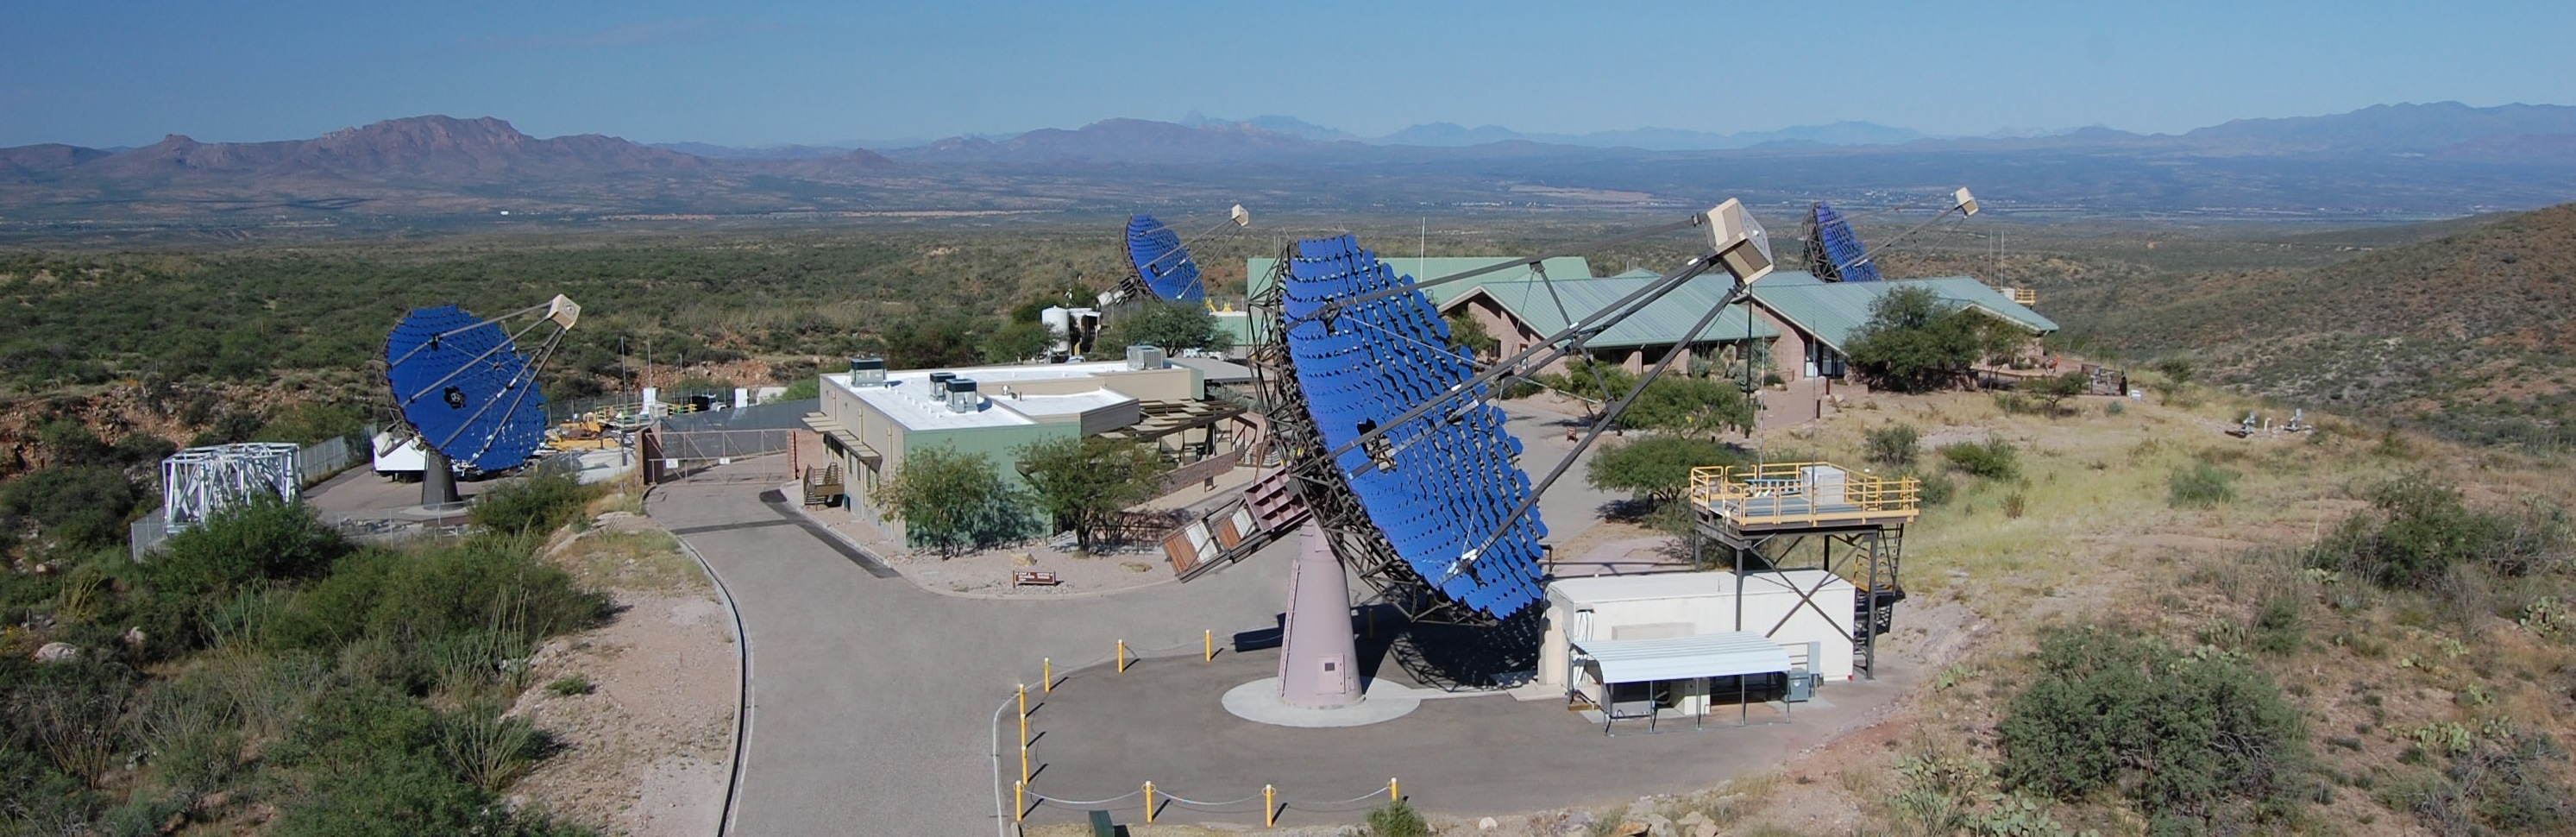
\includegraphics[width=0.8\linewidth]{veritas.jpg}
	\caption[Fred Lawrence Whipple Observatory]{Fred Lawrence Whipple Observatory. Source : \cite{Veritas}}
\end{figure}

\subsection{HAWC}
HAWC pour \textbf{High altitude Water Cherenkov gamma-ray observatory} est un observatoire situé sur le flanc du volcan Sierra Negra au Mexique, à une altitude de 4100 mètres.
Comme son nom l'indique, il observe la lumière Cherenkov dans de l'eau au lieu de l'atmosphère. Ceci permet d'étudier des rayons gamma de plus haute intensité, de 100GeV à 100TeV. \cite{Hawc}

Au lieu d'utiliser des photomultiplicateurs comme les télescopes précédents, HAWC utilise des compteurs de particules basés sur des scintillateurs.
% TODO refaire phrase
Cette différence de fonctionnement comparé aux \gls{iact} lui permet de meilleures performances dans certains domaines tel le champ de vision mais le rend plus sensible au bruit de fond par exemple :

\begin{table}[tbph!]
	\centering{
		\begin{tabular}{ |c|c|c| }
			\hline
			 & \textbf{Télescope Cherenkov} & \textbf{Détecteur de Pluie Atmosphérique} \\
			\hline
			\textbf{Gamme d'énergie} & Basse (<200 GeV) & Haute (>10TeV) \\
			\hline
			\textbf{Rejet de bruit de fond} & Excellent (>99.7\%) & Modéré (>50\%) \\
			\hline
			\textbf{Champ de vision} & Petit (<2°) & Large (>45°) \\
			\hline 
			\textbf{Disponibilité} & Basse (5\%-10\%) & Haute (>90\%) \\
			\hline
		\end{tabular}
		\caption[Complementary detection characteristics of imaging air Cherenkov telescopes (IACTs) and extensive air shower arrays.]{Complementary detection characteristics of imaging air Cherenkov telescopes (IACTs) and extensive air shower arrays, traduit. Source : \cite{Hawc}}
	}
\end{table}

\begin{figure}[tbph!]
	\centering
	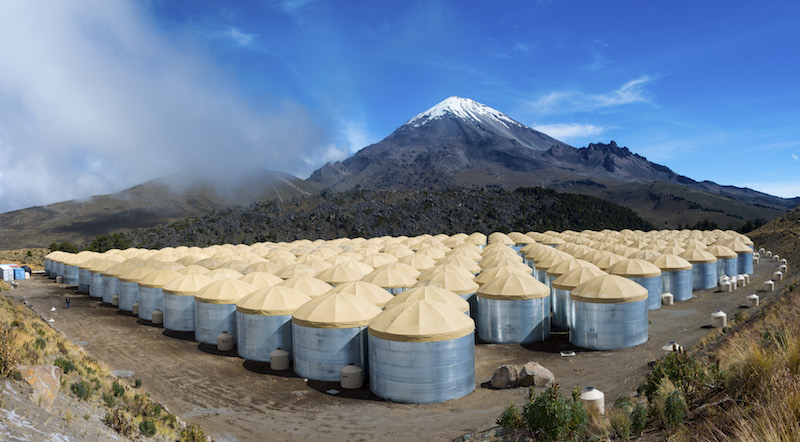
\includegraphics[width=0.6\linewidth]{hawc.jpg}
	\caption[The HAWC Observatory]{The HAWC Observatory. Source : J. Goodman, Nov. 2016 \cite{Hawc}}
\end{figure}

\section{Astronomie gamma future}
\subsection{CTAO}
Le \gls{ctao} est le plus grand projet d'observatoire \gls{iact} au monde. Il est prévu de construire 60 télescopes répartis sur 2 sites, 
le premier (CTAO-North) dans l'hémisphère nord aux îles Canaries sur l'île La Palma et le deuxième (CTAO-South) à Paranal, Chili.

% \begin{figure}[tbph!]
% 	\centering
% 	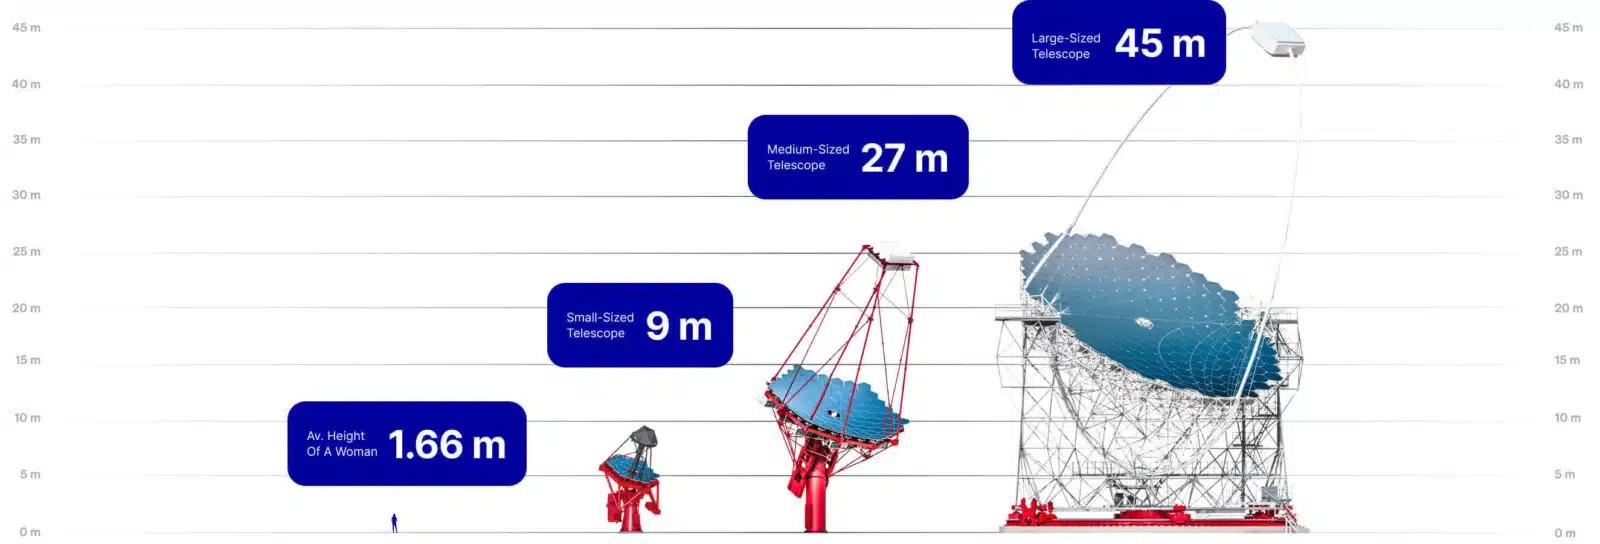
\includegraphics[width=0.8\linewidth]{ctao_telescopes.jpg}
% 	\caption[Illustration des différents télescopes du CTAO]{Illustration des différents télescopes du CTAO. Source : CTAO \cite{Ctao}}
% \end{figure}

L'observatoire est conçu pour étudier les rayons gamma de 20GeV à 300TeV avec plus de 60 télescopes de différentes tailles, \gls{sst}, \gls{mst} et \gls{lst} qui peut atteindre 45m de haut
Pour cela chacun des types de télescopes a été conçu pour répondre au mieux à certaines gammes d'énergie.
Pour la gamme principale de l'installation (150GeV à 5TeV), ce sont 23 \gls{mst} qui sont prévu d'être construire.
37 \gls{sst} sont prévus et ils seront optimisés pour détecter les énergies > 5TeV et jusqu'à 4 \gls{lst} sont prévus pour détecter les gammes d'énergie < 150 GeV.

\begin{figure}[tbph!]
	\centering
	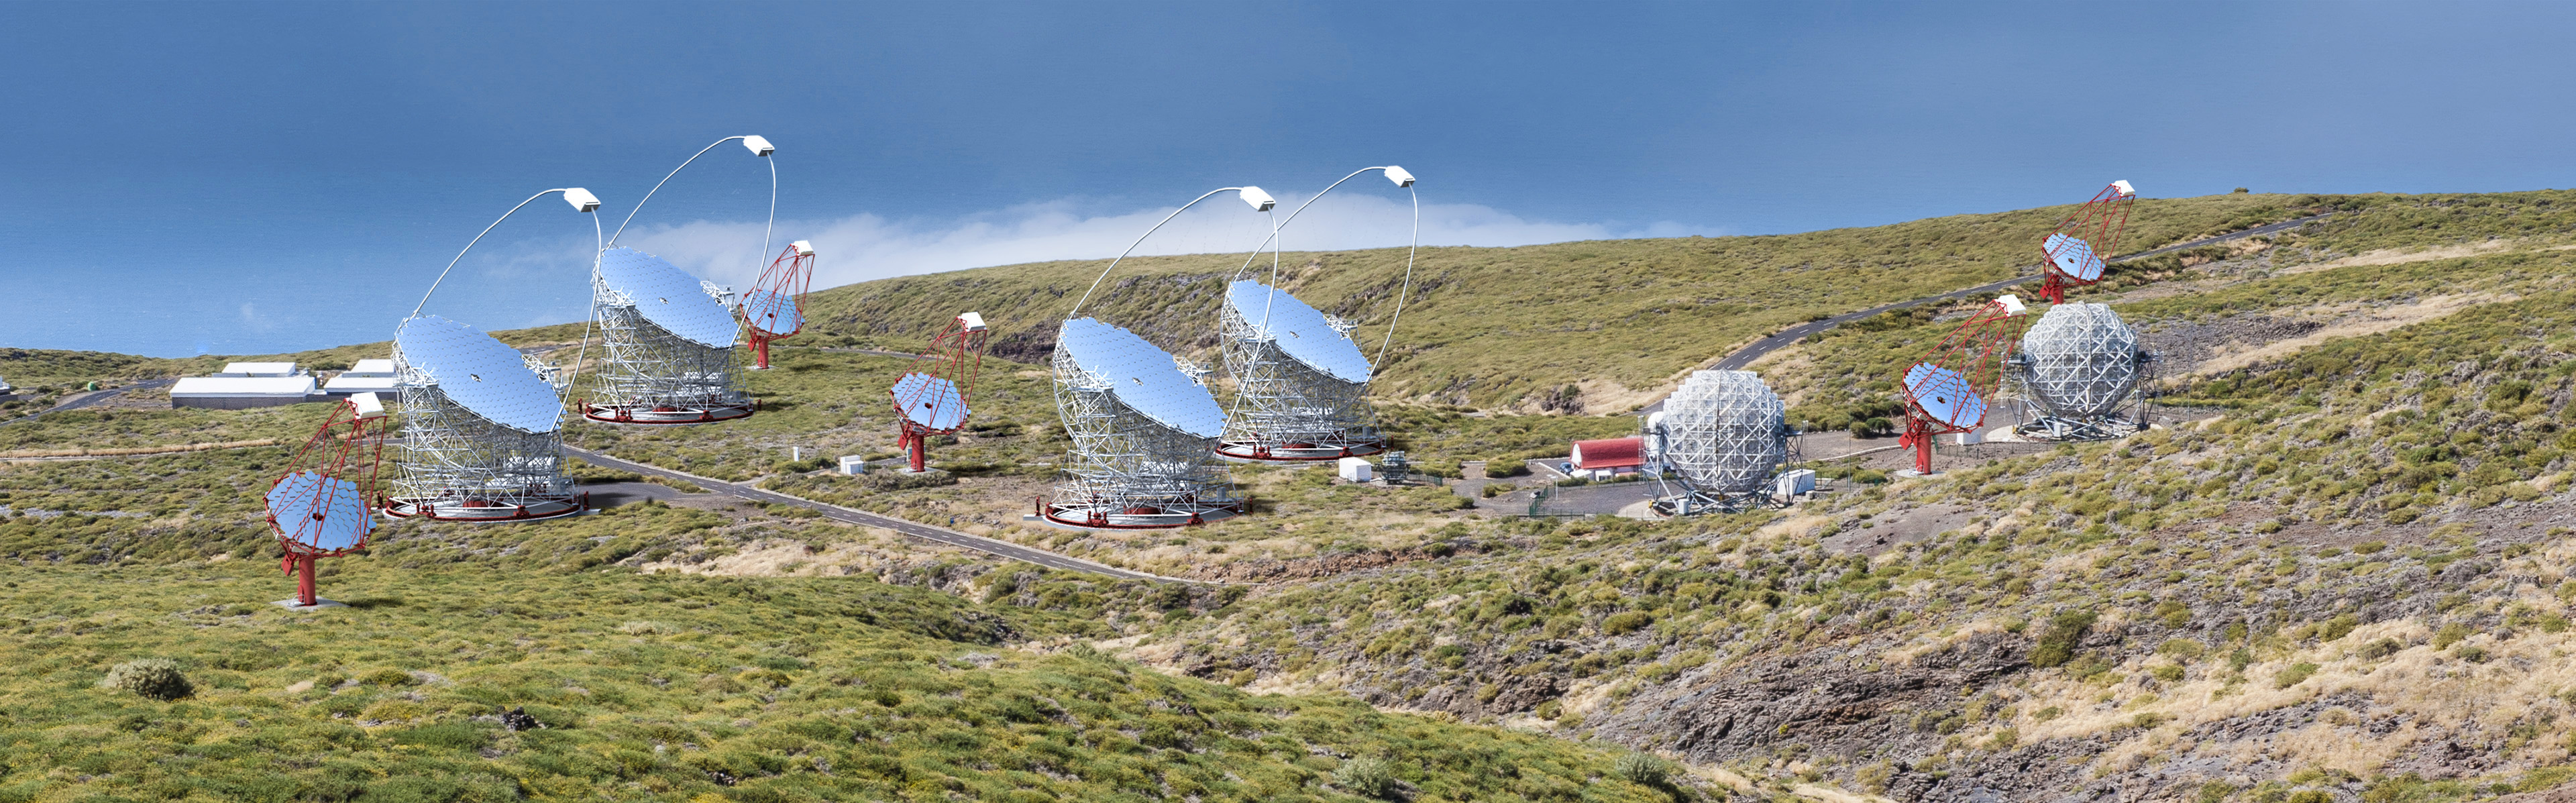
\includegraphics[width=0.9\linewidth]{ctao.jpg}
	\caption[Rendu 3d de CTAO-North]{Rendu 3d de CTAO-North. Source : Gabriel Pérez Díaz, IAC \cite{CtaoImage}}
\end{figure}


% \subsection{ASTRI}